\chapter{Szabályzó kiválasztása és analízise}

Már a modell identifikációját is bonyolította az egynél több bemenet. Illetve kettő van kimenetből is. A szabályzásnál különösen nehéz több bemenetű rendszerre tervezni, esetleg a modellek szétválasztásával lehetséges: külön beavatkozójel a 


Az identifikált modellekre többféle szabályzót tervezek, illetve próbálok ki.

A hasonló feladatokra leggyakrabban modell-prediktív (MPC) szabályzást használnak\cite{AFRAM2014343}. Ehhez szükség van a szakasz modelljére, ami alapján a szabályzó szimulálhatja a szakasz kimenetét. A szimuláció több mintavételi perióduson, egy predikciós horizonton keresztül fut le, minden lehetséges  beavatkozójel-sorozatra a kimenetet szimulálva. Ezen sorozatok közül a legjobbat kiválasztja és egy lépést végrehajt. Ezután a szimuláció újrakezdődik. Az optimális beavatkozójelet egy költségfüggvény minimalizálásával kapja. A költségfüggvényben különböző eltéréseknek vagy abszolútértékeknek különböző súlya lehet.

Egy irodában, vagy lakásban 0.1\si{\celsius}-os vagy 1\si{\celsius}-os pontosságú hőmérsékletszabályzás közötti különbség komfortban aligha érezhető. Ám a követelmények megengedhető mértékű lazítása az energiafogyasztást nagyban lecsökkentheti.

\begin{formal}
	Ha az mpc blokknak van külső ktsg fv. bemenete, használjuk azt. Ebből kössük rá a numerikus képleteket. A teljesítmény integrálját és pillanatértékét, ill. túl gyors változását is lehet büntetni és energetikai szempontotkat (kazán hatásfoka, energia ára, napelemmel megtermelt mennyiség, azaz törés az energiaköltségben, ha egy külön blokkban megadjuk ezeket.)
\end{formal}

\section{Ismerkedés az MPC szabályzással}

\subsection*{Nomenklatúra}

\begin{itemize}[noitemsep,topsep=-8pt,parsep=0pt,partopsep=0pt,leftmargin=42pt]
	\item[\textbf{MPC}] Model Predicive Control
\end{itemize}

\vspace{12pt}


\begin{table*}[h]
	\caption{Az MPC be-és kimenetei a szabályzási körben}
	\label{nomencl_mpcsignals}
	\begin{itemize}[noitemsep,topsep=0pt,parsep=2pt,partopsep=4pt,leftmargin=42pt]
		\item[\textbf{MO}] Measured output of the plant - a visszacsatolt jel
		\item[\textbf{REF}] A referenciajel % konstans vagy tomb?
		\item[\textbf{MD}] Measured disturbance on plant input (?) - ha a zavarjelet lehet mérni, de beavatkozni azon a bemeneten nem lehet
		\item[\textbf{MV}] Manipulated variable of the plant - beavatkozó jel 
	\end{itemize}
\end{table*}
Egyéb MPC paraméterek: mintavételi idő, predikciós horizont, control horizont, súlyozás, soft vagy hard constraintek, cost, optimum (szuboptimum) , stabliltás / garanciák

%terminal constraint, online optimization, adaptive parameters

%\vspace{12pt}


\begin{figure}[h]
	\centering
	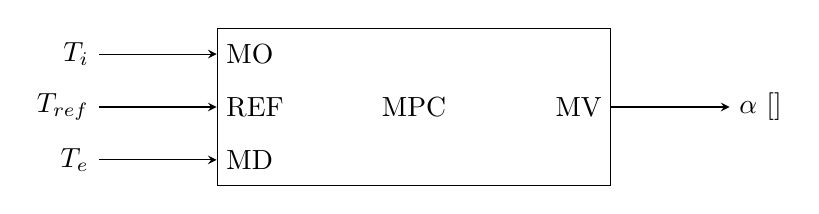
\begin{tikzpicture}[>=stealth]
	% Controller
	% ----------
	\node[draw,rectangle, minimum height=2cm,minimum width=5cm,
		  %label={[xshift=1.0cm, yshift=0.3cm]Label},
		  %label={[xshift=-4.1cm, yshift=-0.7cm]Label},
		  ]
		  (MPC) at (2.3,2.5) {\parbox{2cm}{\centering MPC}};	
	
	% az MPC doboz bemenetei
	\draw [<-] (MPC.165) node[right]{MO} -- +(-15mm,0) node[left]{$T_i$};
	\draw [<-] (MPC.180) node[right]{REF} -- +(-15mm,0) node[left]{$T_{ref}$};
	\draw [->] (MPC.0) node[left]{MV} -- +(15mm,0) node[right]{$\alpha$ [\si{\percent}]};
	\draw [<-] (MPC.195) node[right]{MD} -- +(-15mm,0) node[left]{$T_e$};
	
	\end{tikzpicture}

	\caption{Az MPC be- és kimenetei}
	\label{fig_mpcinout}
\end{figure}


\subsection{Elvárások a szabályzás teljesítményével szemben}

Az MPC hangolása során % működését, tulajdonságait meg tudjam figyelni,
lépésről lépésre fogom módosítani az alapértelmezett paramétereket, azok hatását megfigyelem.
Az MPC szintézis folyamata:% be kellene tabolni


\begin{enumerate}[noitemsep,topsep=0pt,parsep=2pt,partopsep=4pt,leftmargin=30pt]
	\item A szakaszt identifikálni kell, az átviteli függvény be- és kimeneteinek típusát be kell állítani
	\item Létre kell hozni az MPC-t a megfelelő mintavételi frekvenciával
	\item Be kell állítani a jelek fizikai korlátait és súlyukat a szabályzás költségfüggvényében
	%\item Be kell állítani a jelek fizikai korlátait
	\item Hozzá kell adni a Simulink modell Model workspace-éhez a szabályzót és megadni a nevét az Explicit MPC blokkjában. Az itt található Review funciót érdemes használni.
	\item Be kell kötni a jeleket és le kell futtatni a szimulációt
	
\end{enumerate}

%Identifikálni kell a szakaszt.

A \verb|setmpcsignals()| függvény használatával egy új átviteli függvényt hozunk létre, amit az MPC függvénynek odaadhatunk. Ez annyival több az identifikált tf-nél, hogy benne vannak a be-és kimenetek típusai is, aszerint, hogy az említett jelek milyen típusúak. A szakasz átviteli függvényének be-és kimeneteit meg kell nevezni, a típusokat a \ref{nomencl_mpcsignals} listából választhatjuk ki. Ezután az \verb|mpc(tf, Ts)| függvénnyel létrehozhatjuk az MPC szabályzót a megadott szakaszmodellre.

Alapértelmezés szerint a költségfüggvény súlyai az alábbiak. A zárt szabályzási körben ezek a súlyok a hibajelet büntették a legjobban, ezért nagyon jó referenciakövetést sikerült elérni.


Követelmények a referenciajelekre:

Thermal comfort - Olesen, ISO EN 7730

Floor temperature - herz-ől is



%Az MPC szabályzót létrehoztam a toolbox-szal, az identfikált szakaszból. Beállítottam a be-és kimenetek jellegét, korlátait. A ki-és bemeneteket helyesen bekötve már működött is a szabályzás.
%Fontos, hogy helyesen válasszuk meg a mintavételi időt, illetve a súlyokat

%A kezdeti cél egy "sima" szabályzás. Kérdés, hogy egyáltalán tud-e ilyet az MPC. Gyanítom, hogy a hibaminimalizáló függvény megfelelő megadásával tud: ha egy négyzetes hibaminimalizáló van rajta, \textit{biztosan "jó"} lesz.\footnote{Bármit is jelentsen a \textit{jó} szabályzás.}



\subsection{A MATLAB MPC Toolbox elemei}
Az MPC blokknak van egy alapértelmezett költségfüggvénye, és ennek a súlyozását lehet beállítani.
Külön beállítható a szabályzási és a szimulációs horizont.
Ezek optimális beállításai 

A kezdeti MPC szabályzót egyszerűen létre lehet hozni az identifikált modellből és a bemenetek típusának megadásával. (A szelep a beavatkozó jel, illetve a plantnek van még egy bemenete, egy mérhető zavarás.) Ezután a bemenetek értékkészletét adtam meg, illetve van egy normalizáló faktor, ami a jellemző\textit{full scale}.

Az optimalizálás egy költségfüggvény minimalizálását jelenti, amiben \textit{büntetjük} a referenciajeltől való eltérést és a beavatkozó jelek \textbf{értékét vagy változását}.

A fenti a klasszikus MPC, tov. info. Baochang DING, Modern MPC című könyvében olvasható.


%\begin{lstlisting}[
%style=Matlab-editor,
%basicstyle=\mlttfamily,
%escapechar=`,
%]
%tf_19_toMPC=setmpcsignals(tf19, 'Manipulated',[2 3],'MeasuredDisturbances' ,1)
%
%tf_19_toMPC =
%
%From input "u1" to output "y1":
%   3.776e-05 s^2 + 5.958e-09 s + 8.529e-15
%--------------------------------------------
%s^3 + 0.002341 s^2 + 9.301e-09 s + 8.241e-15
%
%
%From input "u2" to output "y1":
%                 7.74 s + 0.000236
%---------------------------------------------------
%s^4 + 1.269e04 s^3 + 4262 s^2 + 3.299 s + 8.454e-06
%
%
%From input "u3" to output "y1":
%  6.361e-05
%-------------
%s + 2.637e-06
%
%Input groups:
%       Name                 Channels
%   Manipulated                 2,3
%     Measured                   1
%
%Output groups:
%       Name                 Channels
%     Measured                   1
%
%Name: tf19
%Continuous-time identified transfer function.
%Parameterization:
%    Number of poles: [3 4 1] Number of zeros: [2 1 0]
%    Number of free coefficients: 14
%    Use "tfdata", "getpvec", "getcov" for parameters and their uncertainties.
%
%Status:
%Estimated using TFEST on time domain data "tf_3in1out__68d".
%Fit to estimation data: 82.28% (stability enforced)
%FPE: 1.707, MSE: 1.706 
%
%
%>> mpc_control_slab=mpc(tf_19_toMPC,1)
%-->Converting linear model from System Identification Toolbox to statespace.
%-->The "PredictionHorizon" property of "mpc" object is empty. Trying
%PredictionHorizon = 10.
%-->The "ControlHorizon" property of the "mpc" object is empty. Assuming 2.
%-->The "Weights.ManipulatedVariables" property of "mpc" object is empty.
%Assuming default 0.00000.
%-->The "Weights.ManipulatedVariablesRate" property of "mpc" object is
%empty. Assuming default 0.10000.
%-->The "Weights.OutputVariables" property of "mpc" object is empty.
%Assuming default 1.00000.
%MPC object (created on 30-Oct-2018 20:51:50):
%---------------------------------------------
%Sampling time: 1 (seconds)
%Prediction Horizon: 10
%Control Horizon: 2
%Plant Model: 
%MATLAB Command Window Page 6
%--------------
%2 manipulated variable(s) -->| 8 states |
%| |--> 1 measured output
%(s)
%1 measured disturbance(s) -->| 3 inputs |
%| |--> 0 unmeasured
%output(s)
%0 unmeasured disturbance(s) -->| 1 outputs |
%--------------
%Indices:
%(input vector) Manipulated variables: [2 3 ]
%Measured disturbances: [1 ]
%(output vector) Measured outputs: [1 ]
%Disturbance and Noise Models:
%Output disturbance model: default (type "getoutdist
%(mpc_control_slab)" for details)
%Measurement noise model: default (unity gain after scaling)
%Weights:
%ManipulatedVariables: [0 0]
%ManipulatedVariablesRate: [0.1000 0.1000]
%OutputVariables: 1
%ECR: 100000
%State Estimation: Default Kalman Filter (type "getEstimator
%(mpc_control_slab)" for details)
%Unconstrained
%>> mpc_control_slab.ManipulatedVariables(1).Min = 0;
%>> mpc_control_slab.ManipulatedVariables(2).Min = 0;
%>> mpc_control_slab.ManipulatedVariables(2).Max = 1;
%mpc_control_slab.ManipulatedVariables(1).Max = 1;
%
%\end{lstlisting}


\subsection{A létrehozott MPC tulajdonságai}

\begin{formal}
	Még lehetséges:
	\begin{itemize}[noitemsep,topsep=-8pt,parsep=0pt,partopsep=0pt]
		%		\item kazán bekapcsolása
		%		\item előremenő hőmérséklet - unmeasured VAGY uncontrolled inputként
		%		\item 1 db. fűtőtest (most radiátor) szelepének tömegárama (szelep áteresztése)
		%		\item Később több fűtőtest vagy többféle fűtőtestek (padlófűtés, különböző teljesítményű radiátorok) szabályozása
		\item környezeti hőmérséklet: predikció / szekvencia használata% is lesz rá. Hatása a kimeneten már identifikálva lett, 3 pólussal és 2 zérussal tökéletesen lekövethető.
		\item napsugárzás zavaró hatása% - szimulálható  a bizonytalansága valószínűleg nagy lesz
	\end{itemize}
	
	Belső változók - fűtési rendszer és ház kapcsolata
	\begin{itemize}[noitemsep,topsep=-6pt,parsep=0pt,partopsep=0pt]
		\item napsugárzás - radiatív, az ablak felületével és a szöggel arányos
		\item fűtőtestek sugárzó és konvektív hőárama
	\end{itemize}
	
	Paraméterek a plantben nem állandók:
	\begin{itemize}[noitemsep,topsep=-6pt,parsep=0pt,partopsep=0pt]
		%		\item hőátadási tényezők hőmérsékletfüggők, áramlási sebesség-függők (szél)
		\item szellőztetés, belső hőterhelés hatása
	\end{itemize}
\end{formal}

%Az elvárás a következő lépésben az, hogy ha egy $t_0$ időpontban a rendszer egy adott állapotban van, és várható egy zavarás $\Delta t$ idő múlva (vagy mértem egy zavarást MOST és a hatása csak később jelenne meg a kimeneten), akkor a rendszer megfelelően beavatkozzon.
%
%(Azaz ha fél óra múlva \SI{10}{\celsius}-al melegebb lesz, ne fűtsön.)

\subsubsection{A kezdeti szabályzó problémái}
Igaz, hogy az alapjelkövetés gyakorlatilag tökéletes volt, de a beavatkozó jelnek a gyakorlatban nem csak a nagysága, hanem a frekvenciája is korlátos. Ezért a beavatkozó szervnek is kell egy átviteli függvény ideális esetben. (Itt most a szelepről van szó.)

A \textit{súlyozatlan} MPC nem vette figyelembe a beavatkozójel változásának \textit{nagy} költségét, ezért irreálisan gyorsan nyitotta és zárta azt.
A gyakorlatban nincs szükség tűpontos referenciakövetésre, a hőmérséklet kb. \SI{1}{\celsius}-ot ingadozhat. ($\pm$ \SI{0.5}{\celsius}) Ha ezt megengedjük, a beavatkozás költsége lecsökkenhet.

\subsubsection{Robosztusság}

A Simulinkben identifikált modellre pontosan lehetett átviteli függvényt illeszteni, így a szabályzóban futó modell gyakorlatilag tökéletes volt. Gyakorlatban viszont a modellek igencsak pontatlanok lehettek, így megvizsgáltam a szabályzás viselkedését megváltozott paraméterekkel is. Ezt a szabályzás alapvetően jól viselte, a referenciakövetés minősége megmaradt.

\section{A szabályzó paramétereinek finomítása, hangolása, alapbeállítások felülírása}

A mintavételi időt megnöveltem. A ház identifikációját és az MPC tervezést is 5 perces időállandóval végeztem. A lépéseket először egy unit test részben hajtottam végre.

\begin{itemize}[noitemsep,topsep=-8pt,parsep=0pt,partopsep=0pt]
	\item A mintavételi idő növelése a Matlab default workspace-ben magával vonja, hogy a Simulink blokkban is módosul a $T_s$. 
	\item A Simulinkben az időt a jobb alsó sarokban mindig mp-ben írja ki. Ámde ha a steppingnél 1000 step-et állítok be, az a jobb alsó sarokban $T_s$-sel felskálázva fogja a mp-t mutatni. Azaz 5 perces sampling time esetén 1 step a jobb alsó sarokban T=300 mp-nek felel meg.
	\item A mintavételi idő megválasztása nagyban meghatározza a költségfüggvény értékét.
%	\item
%	\item
%	\item
%	\item
%	\item
%	\item	
\end{itemize}



\subsubsection{Módosítások az MPC-ben}

A súlyozást módosítva adhatunk költséget a beavatkozásnak, csökkentve így pl. annak a frekvenciáját. Ez a referenciakövetést rontja, de esetünkben nem cél a tized \si{\celsius}-os pontosság, hanem az energiamegtakarítás.
Pontosan fel kellene ezért írni a forintosított költségét a beavatkozásnak, és ezt minimalizálni\footnote{\textit{Model predictive control of radiant slab systems with evaporative cooling sources}, Fang is szelepet használt, de nem értem az ottani optimalizációs algoritmust.}

Egyensúlyt kell találni a referenciakövetés és a beavatkozás között. Külön érdekesség, hogy ha nem távfűtést használunk, akkor a kis beavatkozásnak is nagy költsége van. Erre a súlyozásnál egy LUTot lehetne használni. Btw. a hőszivattyúk kis terhelésen is nagy hatásfokkal működnek. Online weight tune elképzelhető, pl. a beavatkozó jeltől függően.

\subsection{Az MPC költségfüggvénye}




Nem csak a bemenetek értékei súlyozhatók. Az egyik kinyomtatott doksiban nem csak a bemenetek, vagy a hibajel kap súlyozást, hanem a villamos energia aktuális ára is tényező.

Kell keresni egy suitable költségfüggvényt. Illetve megfontolandó lenne vízhőmérsékletre szabályozni, annak a költsége szemléletesebb.

\subsubsection{Súlyozás}
A beavatkozó jelek és a szakasz kimenete is súlyozható, hogy azok a költségfüggvénybe mennyire szóljanak bele. A MATLAB lehetőséget ad arra, hogy ezeket a súlyokat működés közben befolyásoljuk. A Simulinkben beállítottam, hogy a radiátor szelepének alacsony kimenetére a szelep súlya 1 legyen, viszont 30\%-ban kinyitott szelepre csökkenjen le 0.5-re. Ez nem hozott javulást, ugyanis a nagy súllyal az MPC a predikciós horizonton végrehajtott egy optimalizálást. Ám ha a szelepet kinyitotta, a súlyok megváltoztak, így az optimális költségű beavatkozójel is. Viszont ennek éppen elősegítenie kellett volna a szabályzást, ehelyett összezavarta.


Valójában fordítva kell. Kis amplitúdó esetén NULLA pluszköltség még jobban kinyitni ("Szívesen" növekedjen tovább ha még csak kicsit van nyitva.) Csak ha félig van kinyitva, akkor növeljük a költséget.

Sajnos viszont a fenti költségeket nem lehet (nehéz) megfeleltetni forintosított tételeknek.

Fel kellene írni egy ideális scenario-t és ahhoz igazítani a ktsg-fv-t, hogy annak az esetnek a kialakulása legyen valószínűbb.


\subsection{Offline MPC - supervisory control}

\textit{4.4. Approaches without real-time dynamic optimization}\footnote{Thieblemont-ból. A real-time update nélküli MPC a legegyszerűbb és a leggyorsabban kiszámolható. Gyakran más irányítási technikákon alapul.} Döntési fa, affin leképezés ilyenek.

Elkészíteni az offline döntési hálót viszont nehezebb.


	


\subsection{Validálás}
Szimulációval ellenőrizzük a szabályzás robosztusságát. Ehhez megnöveltem a hőtároló tömegeket.

Ötlet: random időpontban lehetne ablaknyitást szimulálni.
Napsütés hatásmechanizmusa.
Radiant heat transfer paramétere továbbra sem olyan világos: sok publikációban a hőmérsékletkülönbség lineáris függését tartalmazza és nem a Stefan-Boltzmann törvény szerinti negyedik hatvány szerintit